% Five-layer resilience architecture diagram
% Label: fig:resilience-architecture
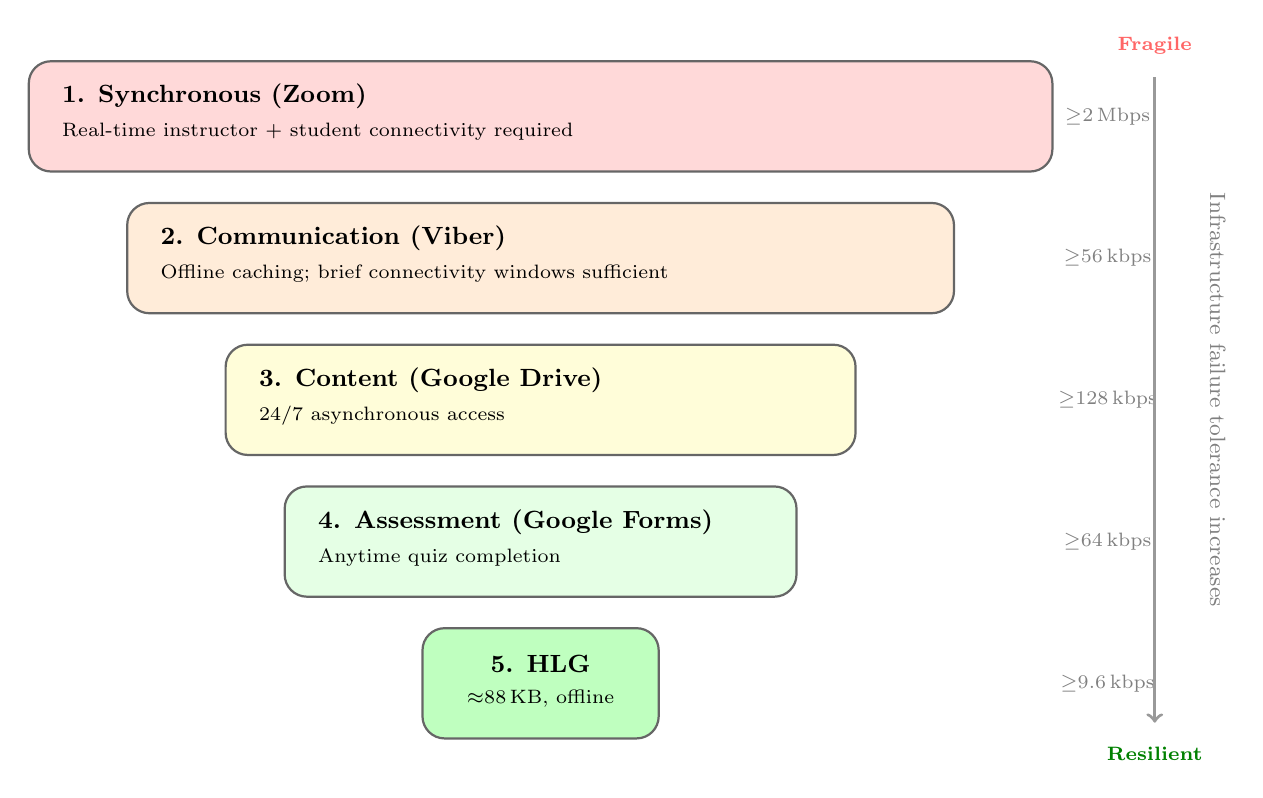
\begin{tikzpicture}[
  layer/.style={rounded corners=8pt, draw=black!60, line width=0.8pt, minimum width=#1, minimum height=1.4cm, align=center, font=\small},
  annot/.style={font=\footnotesize\itshape, text=black!70, align=left},
  bw/.style={font=\scriptsize, text=black!50, align=right}
]

% Layer 5 (outermost, most fragile) — Synchronous
\node[layer=13cm, fill=red!15] (L5) at (0, 0) {};
\node[font=\small\bfseries, anchor=west] at (-6.2, 0.25) {1. Synchronous (Zoom)};
\node[font=\scriptsize, anchor=west, text width=8cm] at (-6.2, -0.2) {Real-time instructor + student connectivity required};

% Layer 4 — Communication
\node[layer=10.5cm, fill=orange!15] (L4) at (0, -1.8) {};
\node[font=\small\bfseries, anchor=west] at (-4.95, -1.55) {2. Communication (Viber)};
\node[font=\scriptsize, anchor=west, text width=7cm] at (-4.95, -2.0) {Offline caching; brief connectivity windows sufficient};

% Layer 3 — Content
\node[layer=8cm, fill=yellow!15] (L3) at (0, -3.6) {};
\node[font=\small\bfseries, anchor=west] at (-3.7, -3.35) {3. Content (Google Drive)};
\node[font=\scriptsize, anchor=west, text width=5.5cm] at (-3.7, -3.8) {24/7 asynchronous access};

% Layer 2 — Assessment (widened from 5.5cm to 6.5cm)
\node[layer=6.5cm, fill=green!10] (L2) at (0, -5.4) {};
\node[font=\small\bfseries, anchor=west] at (-2.95, -5.15) {4. Assessment (Google Forms)};
\node[font=\scriptsize, anchor=west, text width=5cm] at (-2.95, -5.6) {Anytime quiz completion};

% Layer 1 (innermost, most resilient) — Gamification
\node[layer=3cm, fill=green!25] (L1) at (0, -7.2) {};
\node[font=\small\bfseries] at (0, -6.95) {5. HLG};
\node[font=\scriptsize] at (0, -7.4) {${\approx}$88\,KB, offline};

% Bandwidth annotations (right side)
\node[bw] at (7.2, 0) {$\geq$2\,Mbps};
\node[bw] at (7.2, -1.8) {$\geq$56\,kbps};
\node[bw] at (7.2, -3.6) {$\geq$128\,kbps};
\node[bw] at (7.2, -5.4) {$\geq$64\,kbps};
\node[bw] at (7.2, -7.2) {$\geq$9.6\,kbps};

% Arrow: failure tolerance increases
\draw[->, very thick, black!40] (7.8, 0.5) -- (7.8, -7.7);
\node[rotate=-90, font=\footnotesize, text=black!50] at (8.6, -3.6) {Infrastructure failure tolerance increases};

% Fragile/Resilient labels
\node[font=\scriptsize\bfseries, text=red!60] at (7.8, 0.9) {Fragile};
\node[font=\scriptsize\bfseries, text=green!50!black] at (7.8, -8.1) {Resilient};

\end{tikzpicture}
